\subsection{Convenience}
As we mentioned earlier, our goal is for the user to have access to the direct data without having to deal with any
of the technical processes involved in implementing a system. The points we must cover to achieve this goal are: \\

\textbf{Infrastructure}. Data collection, processing, storage and visualization. For example, in most cases, the data is
published periodically, but the set of published data only contains the most recent samples, so there is no way to obtain
a history of the data if they are not collected, processed and stored periodically. \\

\textbf{Automation}. As we commented in the previous point, these tasks are repetitive and also tend to be arduous processes, so it will be
necessary to automate it, otherwise the effort required by the user to extract the information will not compensate. \\

\textbf{Availability} To offer data to users in a direct way, it is recommended to use a platform to which the user
be familiar For example, it is more feasible that the user feels more attracted to access the data if it does not require
no installation on your devices. \\

\subsubsection{How to solve it} 
We will have to provide all the mentioned infrastructure to be able to carry out all the steps to complete the path of obtaining the
raw data until offering them to the user in an accessible, relevant and irresistible way.
We will try to free the user from repetitive actions, we will automate all the possible processes, to offer the user the information as soon as possible.
directly possible.
We must offer the information through a platform with which the user is familiar, nowadays the use of websites or mobile applications is very common.
It is advisable to offer all the possible information without having to make the user perform complicated actions and do not require any additional software or hardware.

\subsubsection{How we solve it. Aire Guru} 
Malaga's air quality data set is updated every hour, Aire Guru automates the process of collecting the
data through a CRON job that executes a script implemented in JavaScript periodically. This reads the data from the url, processes them,
clean and store in a MongoDB database. That is to say, it implements all the necessary structure.

Thanks to this infrastructure, the user is able to visualize the evolution of pollutants since 2018. You can also see the exhibition
personal to these pollutant during the same period of time.

In addition, with the automation of processes, the user is able to visualize the pollution in real time of the city of Malaga and specifically in the point
in which it is found. \\

\begin{figure}[ht]
    \centering
    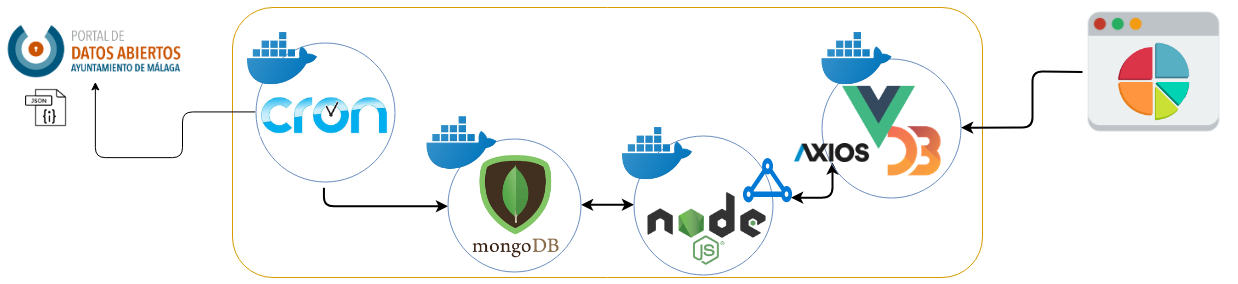
\includegraphics[width=12cm]{aireGuruArquitecture}
    \caption{Arquitecture Aire Guru}
\end{figure}

Through a web interface, it shows the data to the users. \\

\begin{figure}[ht]
    \centering
    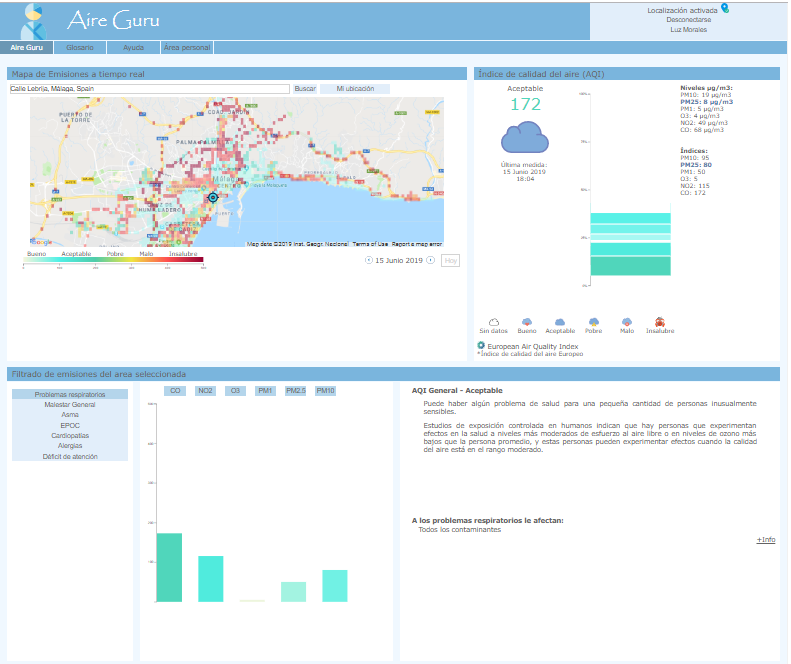
\includegraphics[width=9cm]{aireGuru}
    \caption{Aire Guru. Web Interface}
\end{figure}

To guarantee the reach of the majority of the population, Aire Guru is available at the web addresses https://www.aire.guru and https://www.airquality.guru.
Use SSL that guarantees the encryption of data through the network, more and more browsers try to protect users and
They only show pages that use a secure method.

As we commented previously, all users can see the basic information without having to provide any data or identify themselves, without the need to
perform no download or installation and today, almost everyone is familiar with web browsing.
When we do not force the user to perform extra actions, such as a download or identification, the user will feel less forced to give us an opportunity.


\elsparagraph{Evaluation}  
\begin{itemize}
\done The data necessary for our model have been extracted from the raw data.
\done Infrastructure. It implements all the necessary architecture of storage, processing and visualization so that the user only has to consult
the data.
\done It automates the processes of data collection and the necessary calculations to show the information to the user.
\done Offering users a free web page, facilitates the user to access information directly
\end{itemize}

